\chapter{Cwiczenie 1}

\section{Obsługa oscyloskopu}
\label{sec:obsluga_oscyloskopu}
\begin{itemize}
\item W celu zapoznania się z możliwościami oscyloskopu włączono kanały \textbf{1} oraz \textbf{2} 
\item Ustawiono skalę pionową za pomocą pokrętła znajdującego się poniżej przycisków do włączenia kanałów odpowiednio na \textbf{500 mV} oraz \textbf{100mV}.
\item Skala pozioma została ustawiona na \textbf{10 ns} a tryb wyzwalania na \textbf{AUTO}.
\item Sygnał \textbf{1} (oznaczony na żółto) przesunięto na $\frac{2}{8}$ wysokości ekranu od góry, zaś \textbf{2} (oznaczony na niebiesko) na środek ekranu.
\item Terminacja została ustawiona na \textbf{50$\Omega$} a sprzężenie na \textbf{DC}

\begin{figure}[h]
    \centering
    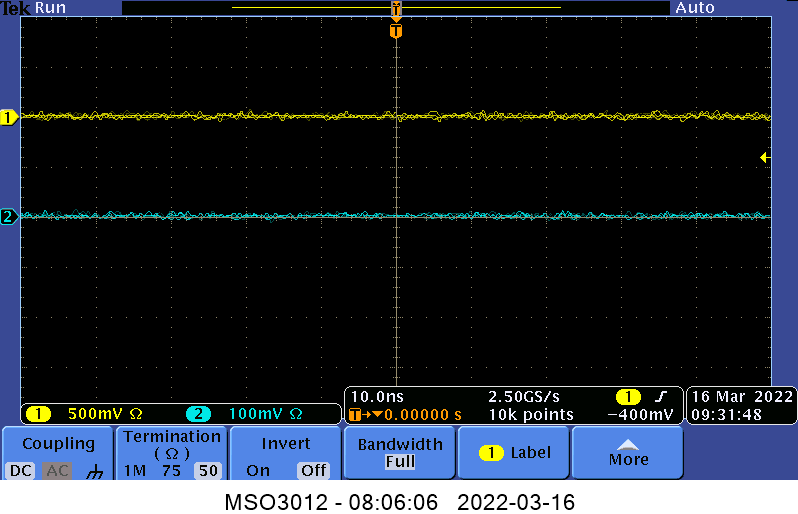
\includegraphics[scale=0.6]{images/1_1_wmenu_smaller.png}
    \caption{Obsługa oscyloskopu - podstawowe ustawienia}
    \label{fig:1_1}
\end{figure}
\end{itemize}

\section{Obsługa generatora funkcyjnego}

W celu zapoznania się z obsługą generatora funkcyjnego podano na oscyloskop sygnał trójkątny o wybranej amplitudzie i częstotliwości.


\begin{itemize}
    \item Za pomocą złącza BNC połączono generator funkcyjny z oscyloskopem na \textbf{kanale 2}.
    \item Włączono \textbf{kanał 2} na oscyloskopie.
    \item Za pomocą generatora funkcyjnego podano \textbf{sygnał trójkątny} wybrany z menu generatora (\textbf{panel Function})
    \item Za pomocą przycisków znajdujących się po prawej stronie wyświetlacza generatora ustawiono \textbf{amplitudę} sygnału na \textbf{1.55V} a jego \textbf{częstotliwość} na \textbf{15kHz}
    \item Powiększono sygnał na oscyloskopie
\end{itemize}

\begin{figure}[h]
    \centering
    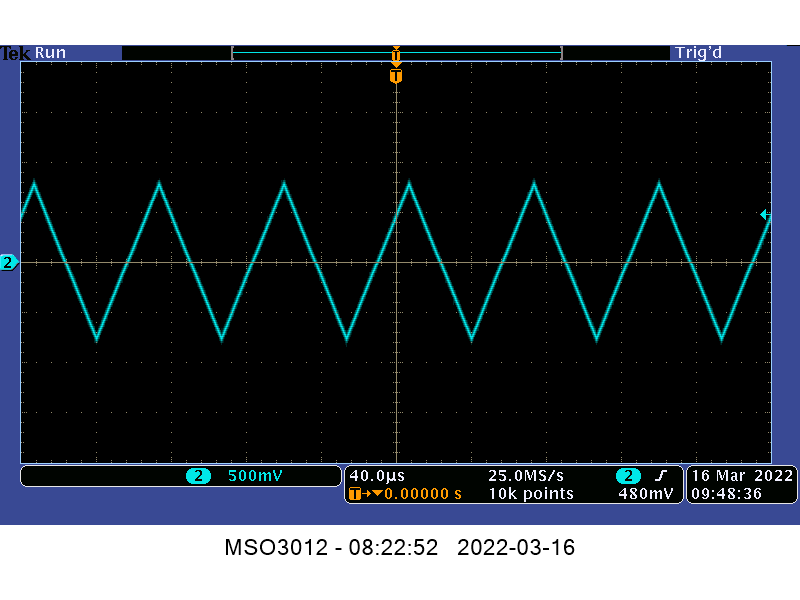
\includegraphics[scale=0.5]{images/1_2.png}
    \caption{Sygnał trójkątny - 1.55V 15kHz}
    \label{fig:trojkat}
\end{figure}

\section{Pomiary}

Dokonano pomiaru podanego przez generator funkcyjny sygnału na \textbf{kanale 2} za pomocą trzech metod.

\label{ad:roznica_2_3-1}
\begin{enumerate}
    \item Metoda określona jako \textbf{pomiar 'na oko'} - za pomocą skali poziomej możemy określić amplitudę podanego sygnału. Skala pozioma została ustawiona na \textbf{500mV} po czym zauważono że sygnał rozpina się na $\frac{3}{8}$ wysokości ekranu. (rys. \ref{fig:trojkat})
    \begin{center}
        Zmierzona wartość = skala $\cdot$ wysokość na ekranie \\
        Zmierzona wartość = 500mV $\cdot$ 3 = 1.5V \\
    \end{center}
        \textcolor{purple}{Różnica wartości wysłanej oraz zmierzonej wyniosła:} 
    \begin{center}
        \textcolor{purple}{$\Delta$ = Teoretyczna wartość - Zmierzona wartość \\ $\Delta$ = |1.55V - 1.5V| =} 0.05V = 50mV
    \end{center}
    
    \item Pomiar za pomocą kursorów - kursory włączono za pomocą przycisku \textbf{Cursors} znajdującego się w lewym górnym rogu menu oscyloskopu. Kursory ustawiono za pomocą pokręteł znajdujących się obok przycisku włączającego kursory (\textbf{multipurpose a/b}) odpowiednio dla mierzonych wartości. W przypadku amplitudy mierzono odległość od najniższego do najwyższego punktu, zaś dla częstotliwości mierzono 1 okres - tutaj od 'dołku' do 'dołku'.
    
    \item Pomiar za pomocą wbudowanych funkcji oscyloskopu - włączone zostały za pomocą przycisku \textbf{Measure} w panelu \textbf{Wave Inspector}, następnie korzystając z nieopisanych przycisków obok wyświetlacza oscylatora wybrano opcję mierzenia \textbf{amplitudy (amplitude)} oraz \textbf{częstotliwości (frequency)} dla \textbf{kanału 2}
\end{enumerate}

\begin{figure}[h]
    \centering
    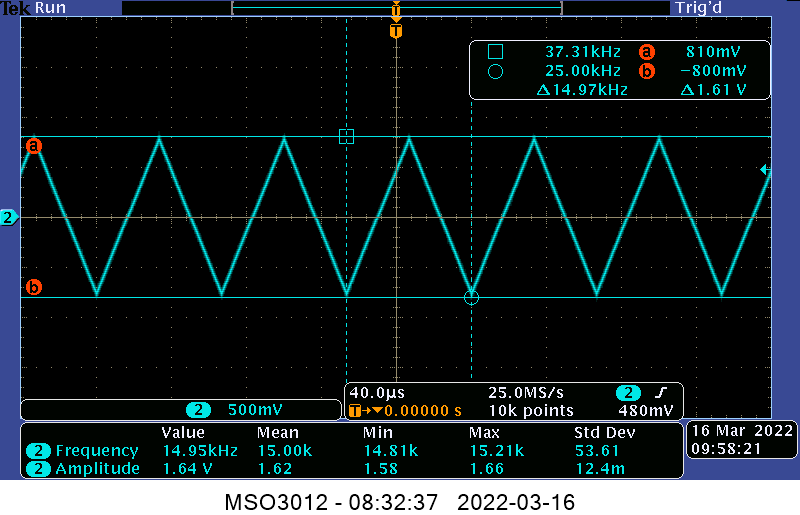
\includegraphics[scale = 0.5]{images/1_3measurement_smaller.png}
    \caption{(\ref{fig:trojkat}) wraz z pomiarami za pomocą kursorów i funkcji wbudowanych}
    \label{fig:trojkat_pomiary}
\end{figure}

\begin{itemize}
    \item W przypadku pomiaru za pomocą kursorów otrzymano następujące wyniki (prawy górny róg \ref{fig:trojkat_pomiary}):
    \begin{center}
        częstotliwość = \textbf{14.97kHz} \\
        amplituda = \textbf{1.61V}
    \end{center}
    \label{ad:roznica_2_3-2}
    \textcolor{purple}{Różnica wartości wysłanych z generatora oraz zmierzonych wyniosła}:
    \begin{center}
        $\Delta$ częstotliwości = \textcolor{purple}{|15kHz - 14.97kHz| =} 0.03kHz = \textbf{30Hz} \\
        $\Delta$ amplitudy = \textcolor{purple}{|1.55V - 1.61V| =} 0.06V = \textbf{60mV}
    \end{center}
    
    \item Pomiar za pomocą funkcji wbudowanych (dolna część \eqref{fig:trojkat_pomiary}):
    \begin{center}
        częstotliwość = \textcolor{purple}{\textbf{15kHz}} \\
        amplituda = \textcolor{purple}{\textbf{1.62V}}
    \end{center}
    \textcolor{purple}{Różnica wartości wysłanych z generatora oraz zmierzonych wyniosła}:
    \label{ad:roznica_2_3-3}
    \begin{center}
        \label{ad:odczyt_2_3}
        $\Delta$ częstotliwości = \textcolor{purple}{|15kHz - 15kHz| = \textbf{0Hz}} \\
        $\Delta$ amplitudy = \textcolor{purple}{|1.55V - 1.62V| = 0.07V} = \textcolor{purple}{\textbf{70mV}}
    \end{center}
\end{itemize}

\section {Zadanie praktyczne - pomiary}

\begin{itemize}
    \item Na \textbf{kanał 1} podano \textbf{sygnał sinusoidalny} o częstotliwości \textbf{15kHz} i amplitudzie \textbf{1V} oraz przesunięciu \textbf{fazowym 30\boldsymbol{\degree}} ($\frac{\pi}{6}$), zaś na\textbf{ kanale 2} podano \textbf{sygnał trójkątny} z poprzedniej części - \textbf{15kHz}, \textbf{1.55V}
    \item Dokonano pomiarów za pomocą kursorów oraz funkcji wbudowanych
\end{itemize}


\begin{itemize}
    \item Za pomocą funkcji wbudowanych w oscyloskopie zmierzono przesunięcie fazowe między \textbf{1} kanałem a \textbf{2}. Zmierzona wartość wyniosła \textbf{31.58}\boldsymbol{\degree}.\\
    \label{ad:roznica_2_4}
    Różnica wartości wyniosła $\approx$ \textcolor{purple}{|30\degree = 31.58\degree| = } \textbf{1.58}\boldsymbol{\degree}.
    
    \begin{figure}[h]
        \centering
        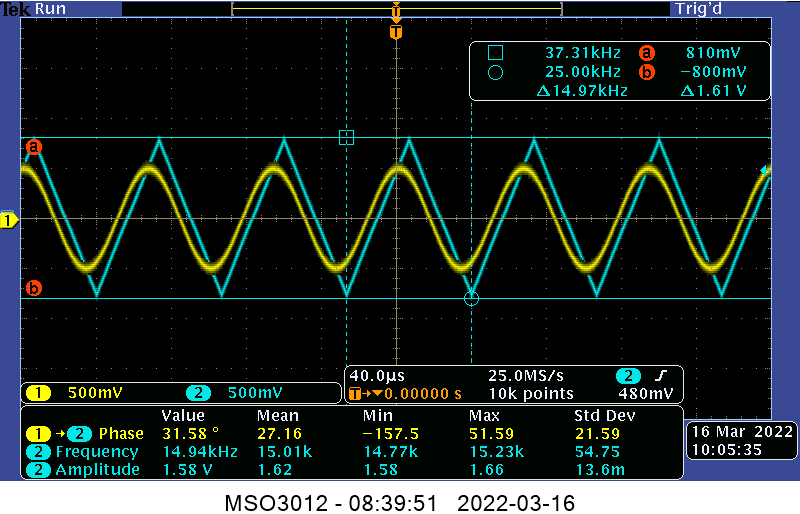
\includegraphics[scale = 0.3]{images/1_4_smaller.png}
        \caption{Sygnał trójkątny oraz sinusoidalny z przesunięciem fazowym 30\degree}
        \label{fig:trójkat_sinus}
    \end{figure}
    
    \item Następnie zmierzono wartości sygnału na \textbf{kanale 1}.
    \begin{center}
        częstotliwość = \textbf{15.06kHz} \\
        amplituda = \textbf{1.1V}
    \end{center}
    \textcolor{purple}{Różnica wartości wysłanych z generatora oraz zmierzonych wyniosła}:
    \begin{center}
        częstotliwość $\approx$ 0.06kHz = \textbf{60Hz} \\
        amplituda $\approx$ 0.1V = \textbf{100mV}
    \end{center}
    
    \begin{figure}[h]
        \centering
        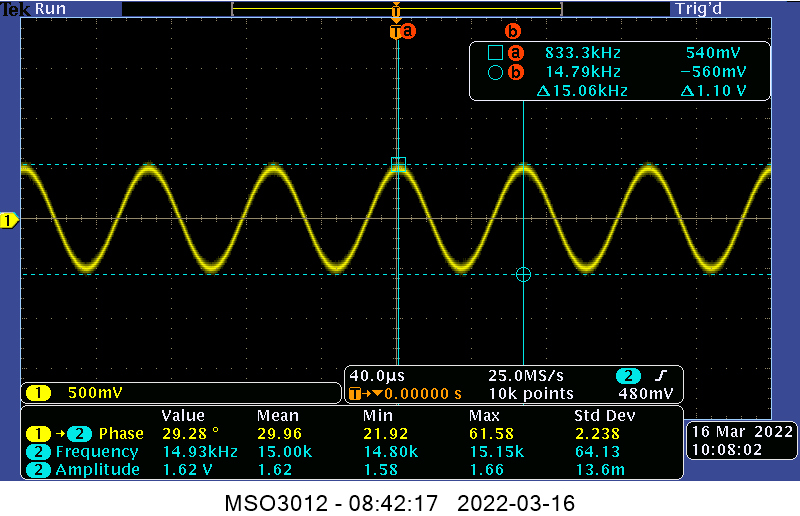
\includegraphics[scale=0.3]{images/1_4sine_smaller.png}
        \caption{Sygnał sinusoidalny wraz z pomiarem za pomocą kursorów}
        \label{fig:pomiar_sinus}
    \end{figure}
\end{itemize}

\section{Podsumowanie}

\begin{itemize}
    \item \textcolor{purple}{Oscyloskop} posiada wiele funkcji ułatwiających dokładny pomiar poprzez dostosowanie skali poziomej oraz pionowej lub zmianę położenia sygnałów
    \label{ad:zla_nazwa_sprzetu_2_5}
    \item Generator funkcyjny w prosty sposób pozwala przesłać na wybrany przez nas kanał sygnał o zadanych parametrach oraz kształcie
    \item Pomiary dokonane za pomocą funkcji wbudowanych jak również kursorów generują w większości niewielkie błędy (różnice między wysłanym sygnałem a zmierzoną wartością)
    \item Posługując się pomiarami za pomocą funkcji wbudowanych w oscyloskopie wykluczamy błędy popełnione przez człowieka, jedynym problemem może być źle skalibrowany sprzęt
    \item Posługując się pomiarami za pomocą kursorów niedokładność pomiarów wynika ze złego ustawienia kursorów, na którą składa się kilka czynników w tym rozdzielczość wyświetlacza na oscylatorze i stopień precyzji kursorów
\end{itemize}